% 2009 年江西卷理科第 9 题：正四面体 ABCD 的顶点 A、B、C 分别在两两垂直的三条射线 Ox、Oy、Oz 上。
% 来源 PDF：gaokaomath-src/普通高考/2009/2009江西理.pdf
% SHA-256：64f70e9750ae2736476d825abdc20639c64a2dfe6c22493b64e710108d5c49e7
% 原页：2009江西理.pdf 第 1 页（A3 三栏）第 1 栏，书页码 533。
% 绘制依据：以 O 为原点，OA=OB=OC，正四面体第四顶点为 D=A+B+C（向量和），
%   故 CD、BD、AD、AC、AB 中，从原页看 CB 与 AD 为虚线（被遮挡），OB 段亦为虚线；
%   OA、OC 两段为实线。斜投影取 Oz 竖直向上、Oy 水平向右、Ox 向右下。
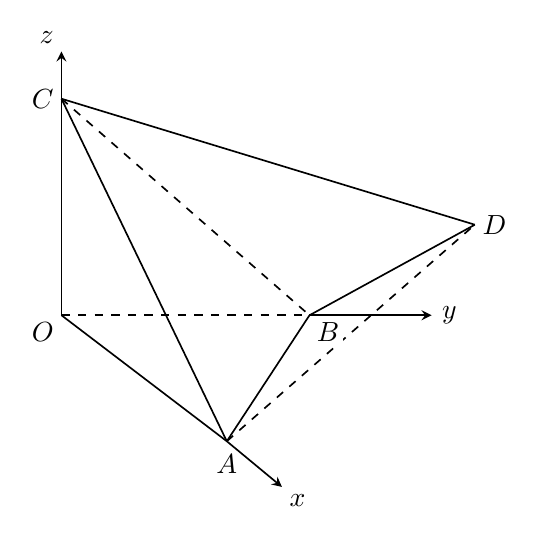
\begin{tikzpicture}[scale=1.0, semithick, every node/.style={inner sep=1.5pt}]
  \coordinate (O) at (2.20,2.60);
  \coordinate (C) at (2.20,5.35);
  \coordinate (B) at (5.35,2.60);
  \coordinate (A) at (4.30,1.00);
  \coordinate (D) at (7.45,3.75);

  % 三条两两垂直的射线
  \draw[->,>=stealth] (O) -- (2.20,5.95);
  \draw[dashed] (O) -- (B);
  \draw[->,>=stealth] (B) -- (6.90,2.60);
  \draw[->,>=stealth] (O) -- (A) -- (5.00,0.42);

  % 正四面体的棱：实线为可见棱，虚线为被遮挡棱
  \draw (C) -- (A);
  \draw (C) -- (D);
  \draw (A) -- (B);
  \draw (B) -- (D);
  \draw[dashed] (C) -- (B);
  \draw[dashed] (A) -- (D);

  \node[above left=1pt] at (2.20,5.95) {$z$};
  \node[left=1pt] at (C) {$C$};
  \node[below left=1pt] at (O) {$O$};
  \node[below=3pt] at (A) {$A$};
  \node[below right=1pt, fill=white, inner sep=1.4pt] at (B) {$B$};
  \node[right=1pt] at (D) {$D$};
  \node[right=2pt] at (6.90,2.60) {$y$};
  \node[below right=1pt] at (5.00,0.42) {$x$};
\end{tikzpicture}
